
\begin{table*}[t]
\centering
\resizebox{0.65\linewidth}{!}{
    \begin{tabular}{@{}lcccccc}
        \toprule
        \multirow{2}[2]{*}{\textbf{{Method}}} & \multicolumn{4}{c}{\textbf{IF=100}} & \multirow{2}[2]{*}{\textbf{{50}}} & \multirow{2}[2]{*}{\textbf{{10}}} \\
        \cmidrule{2-5}
        & \textbf{Many} & \textbf{Medium} & \textbf{Few} & \textbf{All} & & \\
        \midrule
        CE~\cite{cui2019class}                         & 68.31 & 36.88 & 4.87 & 37.96 & 43.54 & 59.50 \\
        \cmidrule{1-7}
        SSD~\cite{li2021self}                          & - & - & - & 46.0 & 50.5 & 62.3 \\
        PaCo~\cite{cui2021parametric}                  & - & - & - & 52.0 & 56.0 & 64.2 \\
        RISDA~\cite{chen2022imagine}                   & - & - & - & 50.16 & 53.84 & 62.38 \\
        CE + CMO~\cite{park2022majority}               & 70.4 & 42.5 & 14.4 & 43.9 & 48.3 & 59.5 \\
        LDAM + CMO~\cite{park2022majority}             & 61.5 & 48.6 & 28.8 & 47.2 & 51.7 & 58.4 \\
        RIDE (3 experts) + CMO~\cite{park2022majority} & - & - & - & 50.0 & 53.0 & 60.2 \\
        Weight Balancing~\cite{alshammari2022long}     & 72.60 & 51.86 & 32.63 & 53.35 & 57.71 & 68.67 \\
        \cmidrule{1-7}
        % Web crawled images                        & 72.71 & 51.21 & 36.13 & 54.06 & 56.40 & 63.86 \\
        % \cmidrule{1-7}
        % Intra-class Image Translation             & 71.86 & 45.88 & 22.97 & 47.87 & 53.33 & 64.95 \\
        % Inter-class Image Translation             & 73.49 & 45.77 & 19.00 & 47.17 & 51.33 & 64.11 \\
        % Class Distribution Fitting                & \textbf{74.83} & 50.79 & 26.03 & 51.53 & 55.60 & 65.60 \\
        % \cmidrule{1-7}
        SYNAuG                                    & \textbf{74.06} & \textbf{56.63} & \textbf{42.83} & \textbf{58.59} & \textbf{61.36} & \textbf{69.01} \\
        % SYNAuG                                         & 74.66 & 52.21 & 27.52 & 52.41 & 56.99 & 66.34 \\
        % SYNAuGAttr                                     & 75.23 & 52.15 & 30.58 & 53.54 & 57.09 & 66.66 \\
        % SYNAuG + Mixup                                 & 75.37 & 54.24 & 32.16 & 54.79 & 57.55 & 66.66 \\
        % SYNAuGAttr + Mixup                             & 74.97 & 53.77 & 35.26 & 55.45 & 58.69 & 66.84 \\
        % SYNAuGAttr + classifier re-training            & 74.83 & 52.57 & 33.13 & 54.53 & 57.93 & 66.80 \\
        % SYNAuGAttr + classifier fine-tuning            & 74.43 & 53.26 & 32.97 & 54.58 & 58.26 & 67.24 \\
        % SYNAuGAttr + Mixup + classifier re-training    & 73.97 & 56.26 & 39.10 & 57.31 & 60.34 & 67.90 \\
        % SYNAuGAttr + Mixup + classifier fine-tuning    & 74.06 & 56.63 & 42.83 & 58.59 & 61.36 & 69.01 \\
        \bottomrule 
    \end{tabular}
    }
    \caption{\textbf{Long-tailed recognition performance on CIFAR100-LT.}
    We compare our SYNAuG with recent works in long-tailed recognition.
    We report the Top-1 accuracy (\%) with different imbalance factors, \ie, IF=\{100, 50, 10\}.
    % \textbf{Bold} stands for the highest accuracy in each IF or class.
    }
    \label{tab:cifar100_lt}
\end{table*}

\begin{table}[t]
\centering
\resizebox{1.0\linewidth}{!}{
    \begin{tabular}{@{}lcccc}
        \toprule
        \multirow{2}[2]{*}{\textbf{{Method}}} & \multirow{2}[2]{*}{\textbf{\makecell{Additional\\Data Type}}}& \multicolumn{3}{c}{\textbf{IF}} \\
        \cmidrule{3-5}
        & & \textbf{100} & \textbf{50} & \textbf{10}\\
        \midrule
        CE~\cite{cui2019class} & N/A & 37.96 & 43.54 & 59.50 \\                        
        % & 68.31 & 36.88 & 4.87 & 37.96 & 43.54 & 59.50 \\
        \cmidrule{1-5}
        Web crawled images    & Real & 54.06 & 56.40 & 63.86 \\
        % & 72.71 & 51.21 & 36.13 & 54.06 & 56.40 & 63.86 \\
        \cmidrule{1-5}
        Intra-class Image Translation & Syn. & 47.87 & 53.33 & 64.95 \\
        % & 71.86 & 45.88 & 22.97 & 47.87 & 53.33 & 64.95 \\
        Inter-class Image Translation & Syn. & 47.17 & 51.33 & 64.11 \\
        % & 73.49 & 45.77 & 19.00 & 47.17 & 51.33 & 64.11 \\
        Class Distribution Fitting     & Syn. & 51.53 & 55.60 & 65.60 \\
        % & \textbf{74.83} & 50.79 & 26.03 & 51.53 & 55.60 & 65.60 \\
        \cmidrule{1-5}
        SYNAuG                          & Syn. & \textbf{58.59} & \textbf{61.36} & \textbf{69.01} \\
        % & 74.06 & \textbf{56.63} & \textbf{42.83} & \textbf{58.59} & \textbf{61.36} & \textbf{69.01} \\
        \bottomrule 
    \end{tabular}
    }
    \caption{\textbf{Comparison with the baselines.}
    We use CIFAR100-LT.
    The second column denotes the data type used in uniformization.
    % with different imbalance factors, \ie, IF=\{100, 50, 10\}.
    % \textbf{Bold} stands for the highest accuracy in each IF or class.
    }
    \label{tab:cifar100_lt_baseline}
\end{table}


\begin{table}[t]
\centering
\resizebox{1.0\linewidth}{!}{
    \begin{tabular}{cccccccc}
        \toprule
        \multirow{2}[2]{*}{} & \multirow{2}[2]{*}{\textbf{Modifier}} & \multirow{2}[2]{*}{\textbf{Mixup}} & \multirow{2}[2]{*}{\textbf{Re-train}} & \multirow{2}[2]{*}{\textbf{Finetune}} & \multicolumn{3}{c}{\textbf{IF}} \\ \cmidrule{6-8}
        & & & & & \textbf{100} & \textbf{{50}} & \textbf{{10}} \\
        \midrule
        (a) & & & & & 52.41 & 56.99 & 66.34 \\
        (b) & \checkmark & & & & 53.54 & 57.09 & 66.66 \\
        % (c) & & \checkmark &  & 54.79 & 57.55 & 66.66 \\
        (c) & \checkmark & \checkmark & & & 55.45 & 58.69 & 66.84 \\
        (d) & \checkmark & \checkmark & \checkmark & & 57.31 & 60.34 & 67.90 \\
        (e) & \checkmark & \checkmark & & \checkmark & \textbf{58.59} & \textbf{61.36} & \textbf{69.01} \\
        \bottomrule 
    \end{tabular}
    }
    \caption{\textbf{Ablation study of SYNAuG.} 
    We use CIFAR100-LT.
    Each component, Modifier, Mixup, Re-train, and Finetune, means we use the class-related modifiers in the prompt, use Mixup augmentation during training, and re-train or finetune the last layer after training, respectively.
    (e) stands for our SYNAuG.
    }
    \label{tab:ablation}
\end{table}



\paragraph{Experimental setting.}
We employ two long-tail datasets: CIFAR100-LT~\cite{cao2019learning} and ImageNet100-LT~\cite{jiang2021self}.
CIFAR100-LT and ImageNet100-LT have train sets that are artificially curated to make class imbalance from the original datasets, CIFAR100~\cite{krizhevsky2009learning} and ImageNet100~\cite{tian2020contrastive}.
The test sets for them are the same as the original one.
The classes in the long-tailed datasets are divided into three groups: Many-shot (more than 100 samples), Medium-shot (20-100 samples), and Few-shot (less than 20 samples).
For CIFAR100-LT, the imbalance factor (IF) can be controlled by computing the ratio of samples in the head to tail class, $N_1/N_K$, where $N_k=\left| \mathcal{D}_k\right|$, and $\mathcal{D}_k$ is the set of samples belonging to the class $k\in\{1,\cdots,K\}$.
As the IF value increases, the skewness of the training data becomes more severe, which makes it more challenging.
%When the IF value is large, the skewness of the training data is more severe, which has fewer samples and is more challenging.
We evaluate under the standard IFs of 100, 50, and 10, following~\cite{alshammari2022long}.
We use ResNet32 for CIFAR100-LT and ResNet50 for ImageNet100-LT.
Further details can be found in the supplementary material.


\paragraph{Competing methods and baselines.}
We compare with recent prior arts: SSD~\cite{li2021self} and PaCo~\cite{cui2021parametric} for self-supervised learning, RISDA~\cite{chen2022imagine} and CMO~\cite{park2022majority} for data augmentation, and Weight Balancing~\cite{alshammari2022long} for the rebalance classifier.
They are state-of-the-art in each perspective and propose methods only using 
% limited to 
the original long-tailed data without external data sources.
% As a strong baseline in terms of data supplement perspective, we collect the data from the internet to populate the insufficient samples, named as WebAug.

We present other 
% baselines by using 
variants of generation methods as baselines:
1) Motivated by the recent work~\cite{he2022synthetic} using the few-shot original samples as guidance during the generation process, we first introduce
% For 
\emph{Intra-class Image Translation}, where we use the original samples from the original training data as a class-wise guidance image for generation,
% It is motivated by the recent work~\cite{he2022synthetic} using the few-shot original samples as guidance during the generation process.
2) Inspired by the M2m~\cite{kim2020m2m} translating an image of the major class to the minor class for leveraging the diversity of the majority information, we introduce
% For 
\emph{Inter-class Image Translation}, where we utilize random samples in the dataset as guidance regardless of the class,
% It is inspired by the M2m~\cite{kim2020m2m} translating an image of the major class to the minor class for leveraging the diversity of the majority information.
3) As an advanced version motivated by DreamBooth~\cite{ruiz2022dreambooth}, we fine-tune the diffusion model with the samples in each class to model the class-wise distribution, named \emph{Class Distribution Fitting},
% ,\footnote{During fine-tuning, we add infrequently used text fragment, such as ``pqk'', as a class token before the target class word in the prompt.
% After fine-tuning the generative model, the added text fragment would become a token that includes the class information.
% The fine-tuned generative model generates synthetic samples for populating the training distribution.}
and 4) As a strong baseline, we collect the real data from the internet instead of generating synthetic images, \ie, \emph{Web crawled images}.
Details are in the supplementary material.


\paragraph{Comparison results.}
We compare SYNAuG with the prior arts in \Tref{tab:cifar100_lt}.
Compared to the CE method~\cite{cui2019class} trained with the Cross Entropy loss on the original data, we achieve large improvements when exploiting the generated samples regardless of the skewness of the training data.
Our method also outperforms 
% shows outperformed performance compared to 
most of the competing methods.
This is stunning results in that it
% The results 
suggests 
% demonstrates
that relieving the imbalance from the data point of view is simple but more effective than the conventional complex algorithmic methods.


In \Tref{tab:cifar100_lt_baseline}, we compare our method with our proposed baselines.
Compared to the case that uses real-world web data\footnote{We collected image from Google image search. Google image search returns images very favorable to DNNs, because Google has used CNN-based image search since March 2013~\cite{chen2015webly}. Thus, using web data is analogous to the distillation of a Google internal model, \ie, very strong baseline.}, it shows that the generated images are of sufficient quality to mitigate the class imbalance problem.
Also, we evaluate additional baselines, which apply the variant methods during the generation process.
% explained in \Sref{sec:2.3} during the generation process.
While they are better than training only with the original long-tailed data (CE method~\cite{cui2019class}), the performance is lower than SYNAuG.
The results imply that the domain gap between the original and synthetic data is hard to narrow during the generation process.
Thus, we propose to leverage 
% using
Mixup during training and fine-tuning the classifier as a more straightforward way.
Note that na\"ively applying Mixup to imbalanced data cases is known to be detrimental~\cite{yebin2023textmania}; thus, we distinctively apply Mixup after uniformizing data distribution which makes a noticeable difference.


\paragraph{Ablation study.}
In \Tref{tab:ablation}, we conduct an ablation study to investigate the influence of each component of our SYNAuG.
When we use modifiers in the prompt, we can get diverse generated samples, which result in the gain between (a) and (b).
We can achieve further improvement by utilizing Mixup (c) to interpolate between original and synthetic data, whereby the domain gap is mitigated by bridging two different domain data.
% the mixed-up data acts as a bridge between the two groups, significantly improving performance.
%When we utilize Mixup (c) for interpolating between original and synthetic data, we can achieve further improvement.
%The mixed-up with original data serves as a bridge between the two groups, affecting largely performance improvement.
Despite the domain Mixup, 
% bridging samples,
the classifier still has room to be more adjusted toward the target data.
To do so, we can re-train (d) or fine-tune (e) the last layer on the uniform distribution data sampling from the original training data, \ie, we set the number of samples in each data class to the smallest number of samples in the original long-tail training data class.
% each data class has the smallest number of samples among the original long-tailed training data classes.
As shown in \Tref{tab:ablation}-(d,e),
% the results, 
we can achieve an additional improvement by adjusting the classifier towards the targeted real data and found that fine-tuning is more effective than re-training.
% \wonseok{and fine-tuning is found to be more effective than re-training.}
%but fine-tuning is more effective than re-training.




\begin{figure}
    \centering
    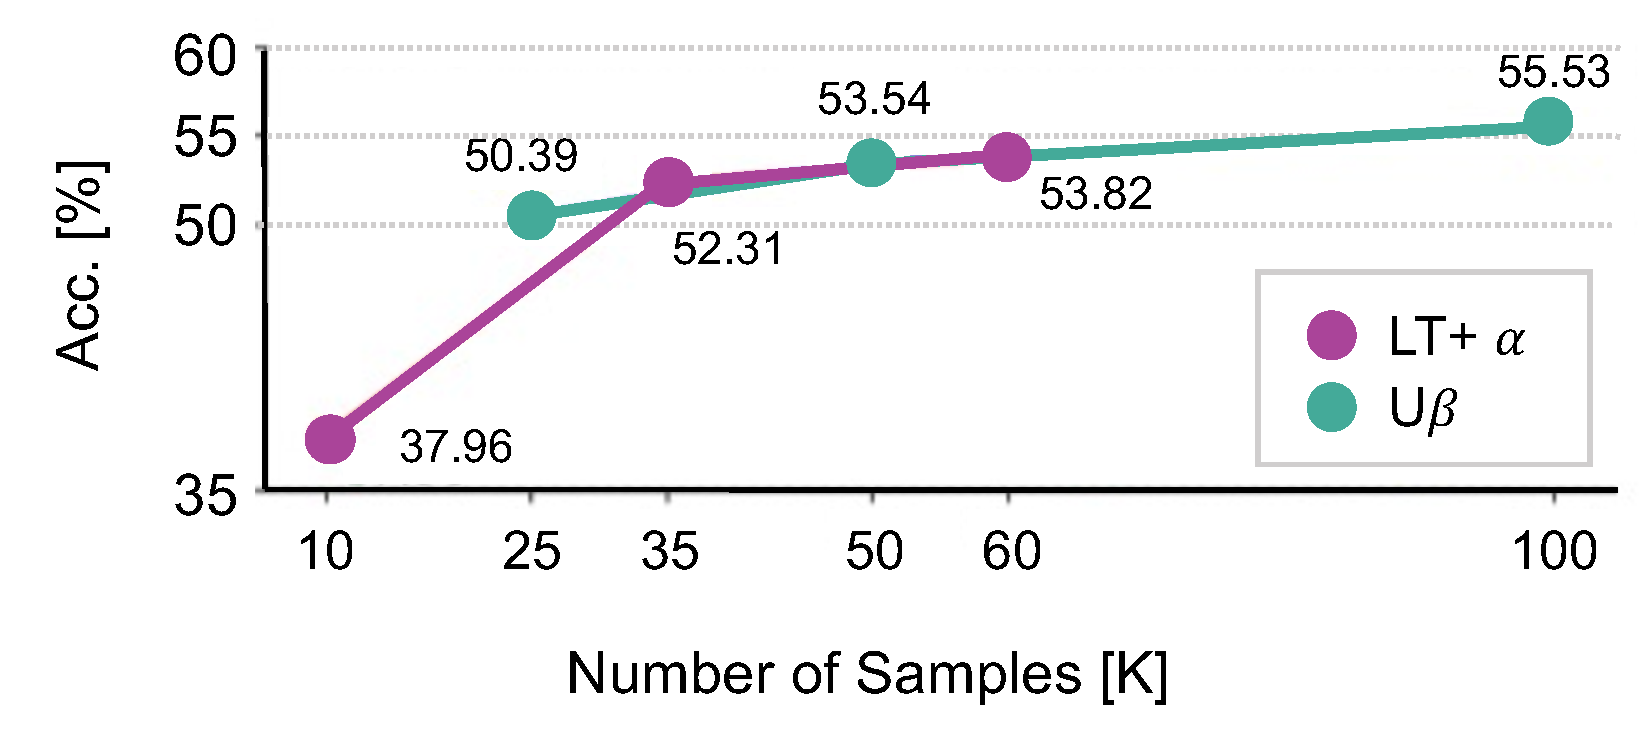
\includegraphics[width=0.95\linewidth]{figures/num_data.pdf}
    \caption{\textbf{Accuracy [\%] (y-axis) vs. number of samples [K] (x-axis).}
    As expected, the performance improves as more synthetic samples are added.
    Additionally, it is improved significantly when the Few class disappears as the number of samples per class increases.}
    \label{fig:alleviate}
\end{figure}



\paragraph{Performance according to the number of synthetic data.}
We explore the performance according to 
% by varying the 
varying number of synthetic data (See \Fref{fig:alleviate}).
We use CIFAR100-LT with the imbalance factor IF=100, \ie, 
% so
the total number of the original samples is 10,847.
%For LT+$\alpha$, we add the synthetic data to all classes equally without care of Many, Medium, and Few classes.
% \wonseok{
For LT+$\alpha$, we uniformly allocate
% incorporate
synthetic data across all classes disregarding the distinction between Many, Medium, and Few classes.
% }
In this case, the absolute difference in sample amount between classes is kept unchanged.
% remains.
%For U$\beta$, we add synthetic data or cut the original samples to be the total number of samples in each class same, \ie, uniformize the data distribution.
% \wonseok{
For U$\beta$, we ensure an equal number of samples in each class by either adding synthetic data or trimming some of the original samples.
% }


% As shown 
In \Fref{fig:alleviate}, the performance is improved as the number of samples increases regardless of the data distribution.
As the quantity of synthetic data increases, accuracies of LT+$\alpha$ and U$\beta$ become quite similar.
%We think that LT+$\alpha$ becomes far from the long-tailed distribution, \ie, the Few class becomes not Few anymore, although the difference in data amount across classes remains in LT+$\alpha$, which reduces the gap between LT+$\alpha$ and U$\beta$.
% 
% \wonseok{
We think that LT+$\alpha$ tends to deviate from the long-tailed distribution as the number
% quantity
of synthetic data increases, \ie, the Few class becomes not Few anymore. Although the disparities 
% variation
in data quantities across classes exist in LT+$\alpha$, this effect diminishes the difference 
% disparity
between LT+$\alpha$ and U$\beta$ with more synthetic data.
% }





\paragraph{Performance according to the quality of synthetic data.}
We evaluate SYNAuG on ImageNet100-LT.
% considering high resolution.
% Since the step value in Stable Diffusion~\cite{rombach2022high} is known to affect the quality of generated images, 
We conduct an ablation study to investigate the impact of data quality of
% different step values
% on
SYNAuG by controlling the diffusion step parameter
% Since the step value in 
of Stable Diffusion~\cite{rombach2022high}, which is known to affect the quality of generated images.
As shown in 
% On the top of
\Fref{fig:imagenet100_lt}-(Top), the generation quality is low when the number of steps is very small, but there is no big difference to the naked eye as it goes up to a certain number.
Figure~\ref{fig:imagenet100_lt}-(Bottom) shows the quantitative results.
% These results lead to quantitative results as well, as shown at the bottom of \Fref{fig:imagenet100_lt}.
Compared to the CE method~\cite{cui2019class} trained on the original long-tailed data, while the accuracy of the Many class is degraded, we achieve large improvement in the Medium, Few, and even All cases
% in all the classes 
regardless of the synthetic image quality.
% Although the accuracy of the Many class is degraded, overall performance, including Medium and Few classes, is drastically improved.
%The results are considerably apart between using synthetic samples with low quality and one with a certain level of quality, but the difference is marginal when the image quality according to the step value exceeds the threshold.
However, there is a certain level of quality that exhibits a surge point in performance.
% The results are 
% considerably different between using synthetic samples with low quality and one with a certain level of quality. 
% However, 
The difference becomes negligible when 
% the image quality according to 
the step value exceeds a certain threshold, \ie, quality.


\begin{figure}[t]
    \begin{subfigure}[c]{0.9\linewidth}
        \centering
        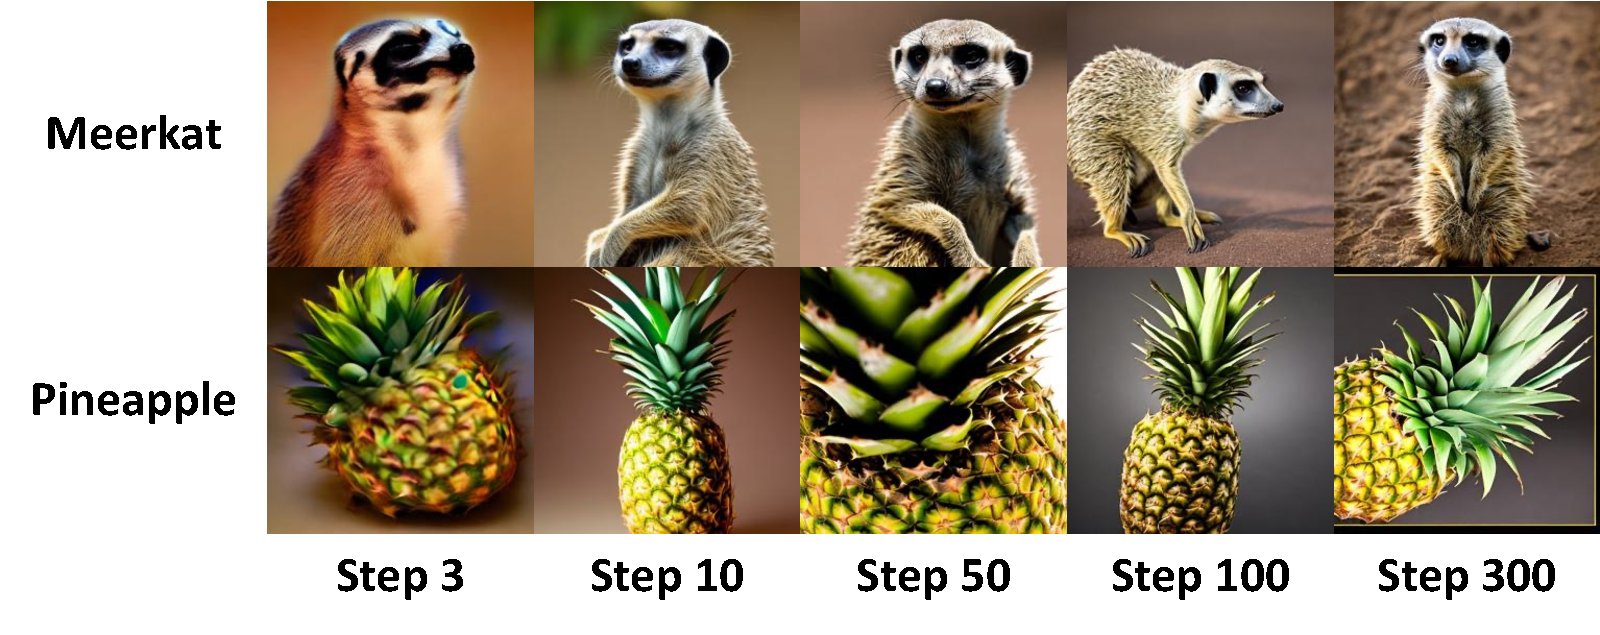
\includegraphics[width=1.0\linewidth]{figures/stepqual_vis.pdf}
    \end{subfigure}
    \centering
    \begin{subtable}[c]{0.9\linewidth}
    \resizebox{1.0\linewidth}{!}{
        \begin{tabular}{@{\,\,\,}lccccc}
            \toprule
            \textbf{Method}  & \textbf{\# step} & \textbf{Many} & \textbf{Medium} & \textbf{Few} & \textbf{All} \\
            \midrule
            CE~\cite{cui2019class}   & & \textbf{61.85} & 15.83 &  0.29 & 32.06 \\
            \cmidrule{1-6}
            \multirow{5}{*}{SYNAuG}
            & 3    & 48.23 & 46.29 & 40.07 & 45.10 \\
            & 10   & 53.89 & \textbf{49.49} & 43.87 & \textbf{49.34} \\
            & 50   & 52.91 & 48.63 & \textbf{45.27} & 49.12 \\
            & 100  & 53.03 & 49.20 & 44.47 & 49.12 \\
            & 300  & 54.11 & 47.71 & 44.73 & 49.06 \\
            \bottomrule 
        \end{tabular}
        }
    \end{subtable}
\caption{\textbf{Ablation study according to sample quality.}
\textbf{(Top)} quality of the generated samples according to the number of steps, \textbf{(Bottom)} long-tailed recognition performance (\%) 
% We report the Top-1 accuracy (\%) 
according to the different times of steps for generating synthetic data, which affects sample quality.
We use ImageNet100-LT with ResNet50.
}
\label{fig:imagenet100_lt}
\end{figure}







